\documentclass[preprint]{revtex4}
%\documentclass[prb,twocolumn]{revtex4}
\usepackage{dcolumn} \usepackage{amsmath} \usepackage{graphicx}
\makeatletter \makeatother

\newcommand{\Kxc}{{\bf K}_{\mathrm{xc}}}
\newcommand{\Np}{N_{\mathrm{p}}} \newcommand{\Nbox}{N_{\mathrm{b}}}
\begin{document}
\title[Short Title]{ Linear scaling computation of the Fock
matrix. VI. Data parallel computation of the exchange-correlation
matrix }

\author{Chee Kwan Gan\footnote{{\tt ckgan@lanl.gov}} and Matt
Challacombe\footnote{{\tt mchalla@lanl.gov}}}
 
\affiliation{ Theoretical Division, Group T-12, MS B268, Los Alamos
National Laboratory, Los Alamos, New Mexico 87545}

\date{Oct 24, 2002}

\begin{abstract}
Recently early onset linear scaling computation of the
exchange-correlation matrix $\Kxc$ essential to density functional
calculations has been proposed and achieved by one of the authors
using Hierarchical Cubature [J. Chem. Phys. {\bf 113}, 10037 (2000)].
Hierarchical Cubature differs from other methods in that it is
adaptive and purely Cartesian, which allows straightforward spatial
decompositions, i.e., the volume enclosing the whole system is simply
divided into a number of non-overlapping boxes. The finite extent of
each box requires only a locally essential density, rather than the
entire density.  This inherent data locality is exploited to reduce
communications between processors as well as to avoid memory and copy
overheads associated with data replication.  Two schemes to partition
the volume of the system (i) the center-of-mass, and (ii) equal-time
partitioning schemes are proposed to achieve a good load balance for
highly irregular parallel computation of $\Kxc$.  The equal-time
partitioning scheme is a measurement based scheme designed to exploit
the temporal locality of the self-consistent-field calculations.
Tests are performed on two systems: (i) taxol, and (ii) a cluster of
110 water molecules. Excellent speedups are obtained. In particular,
we have obtained a 113-fold speedup with 128 processors (i.e., an
efficiency of 88\%) at a very fine-grained level (about one heavy atom
per processor).  For medium-grained calculations, we obtained
superlinear speedups resulting from a combination of good load
balancing and a reduced computational complexity due to data
parallelism.
\end{abstract}

\maketitle

\section{Introduction}
\label{sec:intro}
Density Functional Theory (DFT) and its variant, the hybrid
Hartree-Fock/Density Functional Theory (HF/DFT) have proven to be very
accurate and computationally efficient (compared to those wavefunction
methods~\cite{Kohn_99v71}) that they have been routinely used in
quantum chemistry calculations without compromising accuracy and
reliability~\cite{Becke93,bjohnson93b,Stephens94,Perdew_96v77}. The
recent years have witnessed impressive progress in the algorithmic
developments of $O(N)$ (so-called linear scaling) methods where the
computing time scales linearly with the system size
$N$~\cite{Schwegler96,Challacombe97,%
Scuseria99,Challacombe99,Goedecker99}.  These methods overcome several
computational bottlenecks of $O(N^2)$ to $O(N^3)$, including
computation of the exact Hartree-Fock exchange
matrix~\cite{Schwegler96}, the Coulomb matrix~\cite{Challacombe97},
the exchange-correlation matrix~\cite{Challacombe_00v113}, and
eigensolution of the self-consistent-field
equations~\cite{Challacombe99,Niklasson02}.

The existence of linear scaling methods has been argued from the
concept of ``nearsightedness'' or quantum
locality~\cite{WKohn95,WKohn96}, which implies that the density matrix
$n({\bf r},{\bf r'})$ goes to zero as $|{\bf r}-{\bf r'}| \rightarrow
\infty$. The fundamental reason for this is the loss of quantum phase
coherence between points that are far apart.  Many linear scaling
methods that exploit this decay property have been
proposed~\cite{XLi93,Hernandez96}. It is important to note that
quantum locality also implies data locality, which is an essential
property for scalable parallel algorithms. It should be noted that
successful parallelization of linear scaling methods holds the promise
of very large scale applications, since in principle, with linear
scaling methods an $n$-fold increase in the number of processors
enable the system size to be increased by $n$ times.  However, the
same cannot be said for, say, $O(N^2)$ or $O(N^3)$ methods.  Scalable
parallel algorithms will fully utilize the computing resources that
lie in clusters of personal computers or powerful supercomputers. The
approach to use a cluster of personal computers has proven to be very
cost-effective over the years because the ratio of performance to cost
has been continuously improved. Recently there has been continued
efforts to parallelize quantum chemistry
codes~\cite{Harrison_94v45,Guerra_95,Sosa_98v19,%
Stephan_98v108,Furlani_00v128,Sosa_00v26,Yoshihiro_01v346,Baker_02v23}.

One of most computationally demanding parts of a modern Gaussian
orbital self-consistent-field (SCF) code is numerical integration of
the exchange-correlation potential for DFT or HF/DFT
calculations. Efficient linear scaling approaches have been proposed
to solve this problem~\cite{Challacombe_00v113,Jorda95,Stratmann96}.
Most works~\cite{Furlani_00v128,Jorda95,Stratmann96,Scuseria99} use the idea of
fuzzy polyhedra introduced by Becke~\cite{Becke88}.  These fuzzy
polyhedra are used to create nuclear weight functions so that
integration can be written as a sum of many single-center integrations
centered on atomic nuclei.  Standard numerical techniques are then
used to perform one-center, atomic-like integration in spherical polar
coordinates.  It should be observed that by this transformation, the
singularities due to the cusps at the atomic nuclei are overcome.

A different approach, Hierarchical Cubature (HiCu), has been developed
by Challacombe where an adaptive telescoping Cartesian grid with
cubature rules is used~\cite{Challacombe_00v113}.  In HiCu, the
hierarchical adaptive grids resolve strong variations and multiple
length scales encountered in numerical integration of the
exchange-correlation matrix $\Kxc$.  The $k$-d
tree~\cite{Bentley79,Bentley80,Gaede98} data structure is used to
represent the adaptive grid or CubeTree. The electron density of the
system is also represented by the $k$-d tree data structure, called a
RhoTree.  Each node in a $k$-d tree contains a bounding box (BBox)
that encloses the spatial data contained by it and its children (if
the node is not a leaf node).  Because of the hierarchical
organization of data in a $k$-d tree, a search for all data within a
given Euclidean distance (i.e., a range query) is an efficient
$O(\log_{2}N)$ operation.

The CubeTree is constructed through recursive bisection of a Cartesian
domain (i.e. a box) enclosing the electron density, applying a fixed
fully symmetric $C_3$ (cubature) rules~\cite{Stroud71} within each
BBox.  Given a local error threshold $\tau$, the
recursive bisection process stops when $\delta < \tau$, where
\begin{equation}
\delta = \Delta \rho+ \frac{1}{3} \sqrt{(\Delta \rho_x)^2 + (\Delta
\rho_y)^2 + (\Delta \rho_z)^2}
\label{eq:delta}
\end{equation}
Here $\Delta \rho$ is the magnitude of the difference between the
exact electron charge in the BBox and the numerically integrated
electron charge,
\begin{equation}
\Delta \rho = \left|\int_{\tt{BBox}}\rho({\bf r}) d{\bf r} -
\sum_{i=1}^{N_{\mathrm{g}}} w_i\rho({\bf r}_i)\right|
\end{equation}
where $w_i$ are the grid weights and $N_{\mathrm{g}}$ is the number of
grid points in the cubature rule. The magnitude of the difference
between the analytic and numerical integrations of the $i$th component
(i.e., $i = x$, $y$, or $z$) of the density gradient $\nabla \rho$,
denoted by $\Delta \rho_i $, is calculated in a similar fashion as
$\Delta \rho$.  Unlike the first implementation of
HiCu~\cite{Challacombe_00v113}, our latest HiCu implementation has
incorporated the errors due to the density gradient.  We note that the
accuracy of HiCu can be systematically improved by decreasing $\tau$.
One of the strengths of HiCu is that it displays an early onset of
true linear scaling, even for large basis sets and 3D systems.  The
Cartesian approach of HiCu allows a straightforward domain
decomposition while maintaining data locality.

The main purpose of this work is to efficiently parallelize the
computation of $\Kxc$. We propose a measurement based repartitioning
scheme (called the equal-time partitioning scheme) for domain
decomposition in quantum chemistry, which fully exploits the temporal
locality of the SCF calculations. Temporal
locality means that the workload pattern in the work space (which is
the volume of the system in the case of HiCu) is more or less the same, since the
change in density between SCF cycles is usually small. The inherent data
locality of HiCu is fully utilized to both reduce communications
between processors and memory requirement through a data parallel
approach.

The remainder of this paper is organized as follows.
Section~\ref{sec:parahicu} discusses our strategies to efficiently
parallelize the computation of $\Kxc$ using HiCu.
Section~\ref{sec:data-locality} discusses the issue of data locality
to reduce communications between processors.
Section~\ref{sec:implementation} describes a computational
implementation of data parallel HiCu.  Section~\ref{sec:results}
presents the results and discussions of the speedup tests performed on
two systems. Section~\ref{sec:conclusions} summarizes the main
conclusions of the paper.

\section{Parallelization of HiCu}
\label{sec:parahicu}
In this section we describe the parallelization of HiCu with the goal
of obtaining good speedups even at fine-grained parallelism.  This is
difficult, as computation of the exchange-correlation potential, which
depends on the electron density of the system, is highly irregular for
an inhomogeneous system.  To obtain a good speedup, we need to reduce
both load imbalance and communications between processors. First we
discuss the issue of load balancing. The issue of communication is
discussed in Section~\ref{sec:data-locality}.

Since HiCu is purely Cartesian, spatial decomposition can be performed
by simply sectioning the {\it root BBox} of the RhoTree, which is the BBox
enclosing the entire electron density.  We may arbitrarily partition
the root BBox into $\Nbox$ non-overlapping subboxes.  This suggests a
very naive approach to a dynamic master-slave load balancing scheme
when $\Nbox$ is made much larger than $\Np$ (say, $\Nbox= 4\Np$),
where $\Np$ the number of processors. A master program collects the
results from a slave program which has finished its work on a
particular subbox. The master program then instructs the slave program
to work on a new subbox which has not been assigned to any of the
slave programs before. It should be pointed out that the master-slave
approach has been used to calculate $\Kxc$ in
parallel~\cite{Furlani_00v128,Yoshihiro_01v346} and other quantum
chemistry codes~\cite{Baker_02v23}.

We have tested the simple dynamic master-slave load balancing
scheme. Unfortunately, poor speedups are obtained, especially when
both $\Nbox$ and $\Np$ are large.  This is because as $\Nbox$
increases, the time to deal with a subbox is generally small (since
the volumes are smaller), so most slave programs will finish their
work very quickly and they will spend some time contending for the
master program to respond. This problem is exacerbated by the fact
that the maximum load does not necessarily decrease linearly with
$\Nbox$ due to the irregular nature of the problem, which means a good
speedup may not be obtained even in principle.  It is interesting to
note that Guerra {\it et al.}\/~\cite{Guerra_95} have preferred a
static dynamic load balancing scheme over a master-slave dynamic
load-balance scheme because they found that repeated distribution of
data requires much more communication.

So for massive parallelism, we concluded that a careful domain
decomposition should be made. Since HiCu is intrinsically a tree code,
we have looked into various domain decomposition schemes mostly
related to $N$-body problems~\cite{warren:92_article,Grama94_article,%
Warren95b,Singh93,Singh_95v27,Pilkington96,Grama_98v24}, where most
implementations use a tree data structure (e.g. a quadtree in 2D or an
octree in 3D).  In our case here, we choose to use a static
partitioning scheme where the root BBox is partitioned into $\Nbox =
\Np$ subboxes with the aim of a good load balance.  One may of course
use a larger value for $\Nbox$, but having $\Nbox = \Np$ has the
obvious advantage that each processor needs to deal with one subbox at
most.  We propose a heuristic center-of-mass (COM) partitioning scheme
for the parallel calculation of $\Kxc$ in the very first
self-consistent-field (SCF) cycle.  The COM partitioning scheme will
be explained in subsection~\ref{subsec:COM}.  For all subsequent SCF
cycles after the first SCF cycle, we will repartition the root BBox
using the load information collected in the previous cycle.  The
reason for this repartitioning scheme is as follows.  In a SCF
calculation, the electron density of the system changes from one SCF
cycle to the next.  The grid (CubeTree) for integration of
exchange-correlation potential in each SCF cycle will adapt
automatically to the new density.  Since the change in the electron
density is usually gradual (especially if one starts from a reasonably
good density guess, such as a superposition of atomic densities), and
small near self-consistency, it is of great importance to use the load
information in the previous SCF cycle to repartition the root BBox in
the current SCF cycle. In this way, temporal
locality~\cite{Pilkington96} of the problem will be exploited and load
balance will be continuously improved through repartitioning. This
equal-time (ET) repartitioning scheme will be further explained in
subsection~\ref{subsec:equal-time}.

\subsection{Center-of-mass partitioning scheme}
\label{subsec:COM}
% BEGIN FIGURE
\begin{figure}[t]
\resizebox*{3.5in}{!}{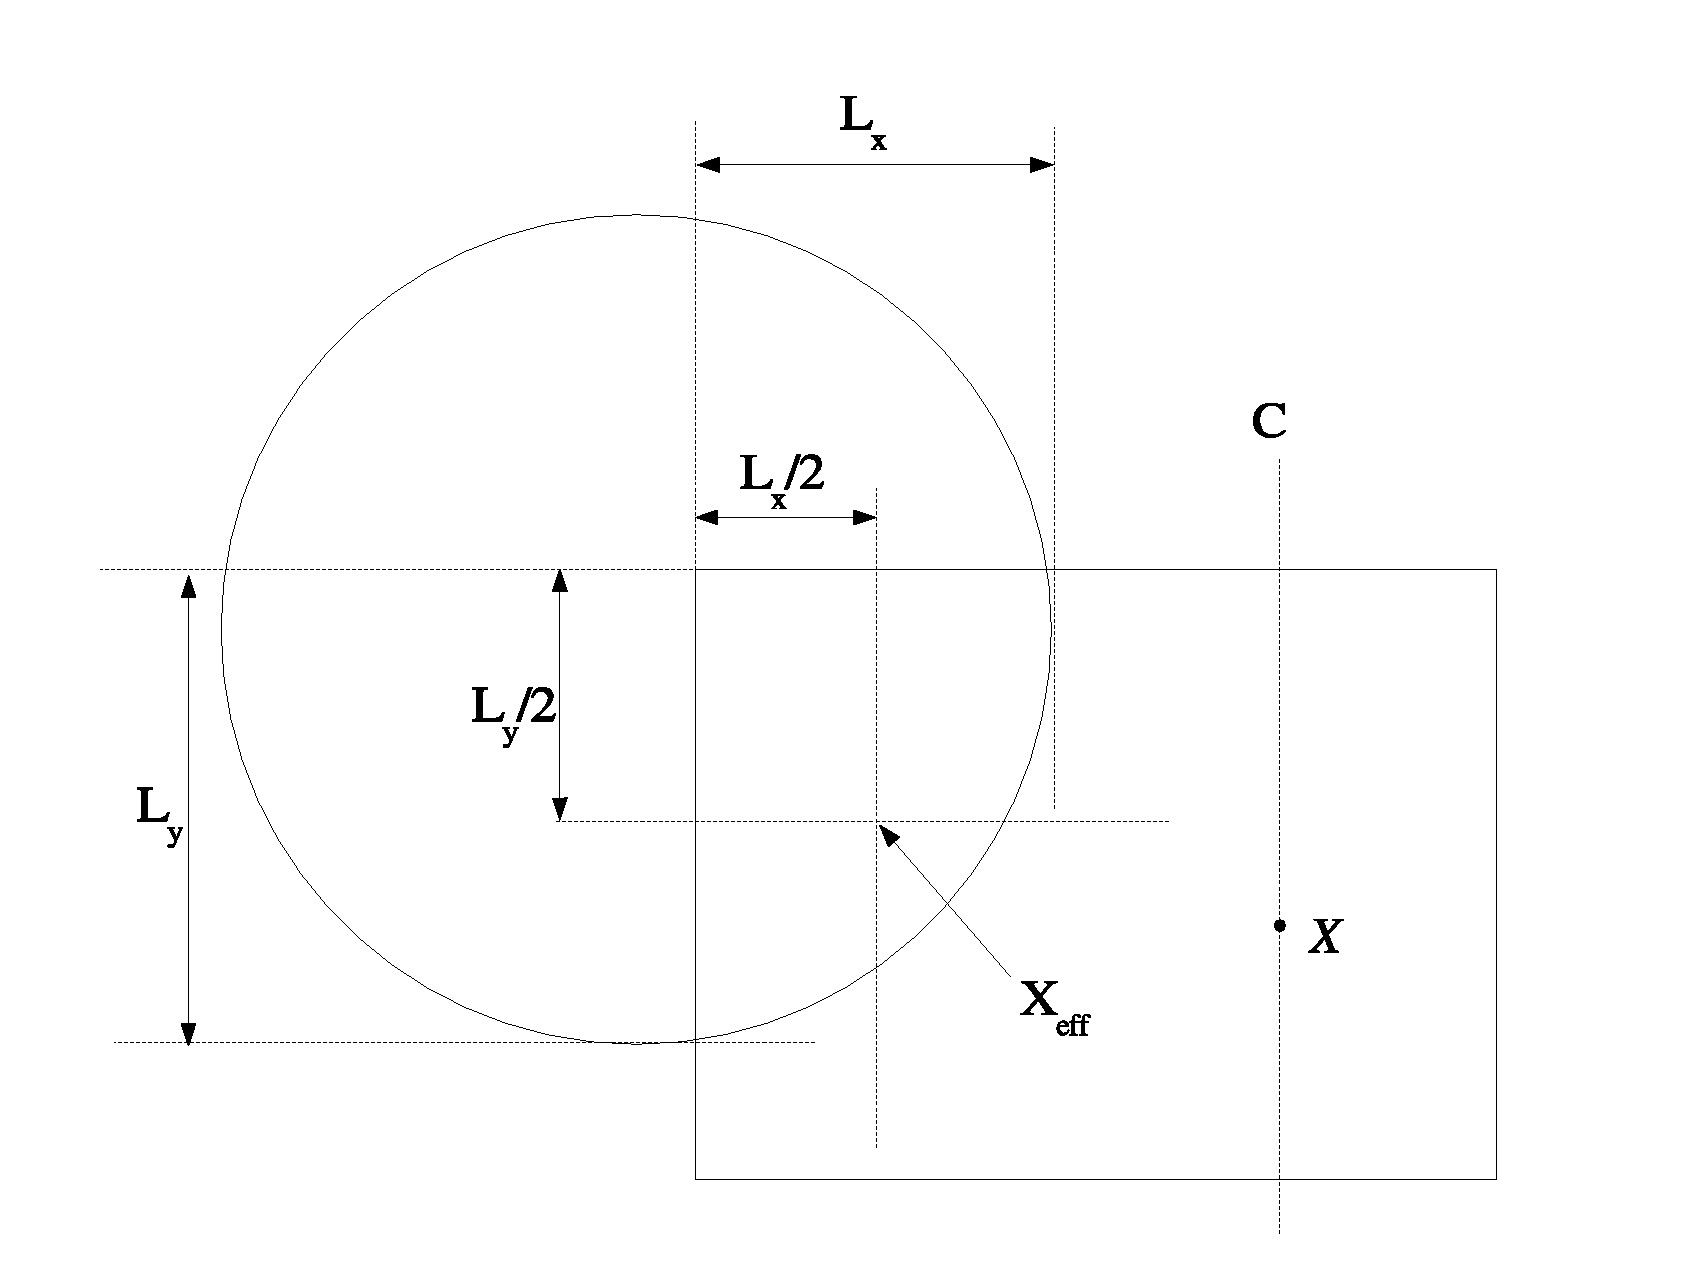
\includegraphics[clip]{COM.eps}}
\caption{ A schematic diagram to explain the center-of-mass (COM)
partitioning scheme.  A sphere of Bragg-Slater~\cite{Slater_64v41}
radius $R_i$ centered on the atom $i$ is drawn for each atom (for
simplicity, only one atom is considered in this case).  The volume of
box-sphere intersection is approximated by $L_x L_y L_z$, where the
$L_x$ is the range of intersection between the sphere and the box in
the $x$ direction. $L_y$ and $L_z$ are calculated in a similar
way. For simplicity we have assumed that the effective charge
$Z_{\mathrm{eff},i}$ is centered at ${\bf X}_{\mathrm{eff}}$. Also
shown is a cutting plane C passing through the center of mass ${\bf
X}$.  }\label{fig:COM}
\end{figure}
% END FIGURE

In the center-of-mass (COM) partitioning scheme, we make a plausible
assumption that the computing time for a subbox is proportional to the
total electron charge in the box.  To partition a BBox (see
Figure~\ref{fig:COM}), we first calculate the center of the electron
charge, which we have loosely called the ``center of mass''.  We
assume that the electron charge due to an atom $i$ is smeared out
evenly in a sphere of radius $R_i$, which we have taken to be the
Bragg-Slater radius~\cite{Slater_64v41} for the atom.  The
Bragg-Slater radius for an atom is the empirical atomic radius,
derived from the fact that two atoms forming a bond in a crystal or
molecule gives an approximate value of the internuclear distance. It
is observed that inter-atomic bond lengths in solids and molecules,
whether ionic or covalent, are approximately equal to pairwise sums of
unique atomic radii~\cite{Slater_64v41}.  The center of mass (charge)
${\bf X}$ is given by
\begin{equation}
{\bf X} = \frac{\sum_{i} Z_{\mathrm{eff},i} {\bf X}_{\mathrm{eff},i}}
{\sum_{i} Z_{\mathrm{eff},i}}
\label{eq:X}
\end{equation}
where $Z_{\mathrm{eff},i} = Z_i (L_x L_y L_z/V_i)$, with $V_i = 4\pi
R_i^3/3$.  The symbols $L_x$, $L_y$, $L_z$, and ${\bf
X}_{\mathrm{eff},i}$ are explained in Figure~\ref{fig:COM}. The index
$i$ in Eq.~(\ref{eq:X}) runs through all atoms which overlap (totally
or partially) with the box to be partitioned.  In practice, we only
calculate one component of ${\bf X}$, which is along the largest
dimension of the box, since only one cutting plane is passing through
${\bf X}$.  Each of the two subboxes after a COM partitioning may be
subjected to another COM partitioning.  For simplicity, we always
partition the root BBox in such a way that the number of the subboxes
is a power of two, even though this restriction can be dropped easily.
In a parallel calculation, only one processor will perform the serial
COM partition and broadcast the dimensions of subboxes to all
other processors. It is important to emphasize that although the COM
partitioning scheme might not give a good load balance, it does serve
as a cheap and good starting partition for parallel HiCu.  This is not
a problem even for a large system because we can use a
reasonably large local error threshold $\tau$ and a minimal basis set
to start a calculation while the equal-time partitioning scheme, to be
explained in subsection~\ref{subsec:equal-time}, will improve the
efficiency in subsequent SCF cycles.  One can then switch to a better
basis set or lower the threshold $\tau$ during the iterative
calculations.  We note that it is possible to use other initial
partitioning schemes to replace COM partitioning scheme.

\subsection{Equal-time partitioning scheme}
\label{subsec:equal-time}
% BEGIN FIGURE
\begin{figure}[t]
\resizebox*{3.5in}{!}{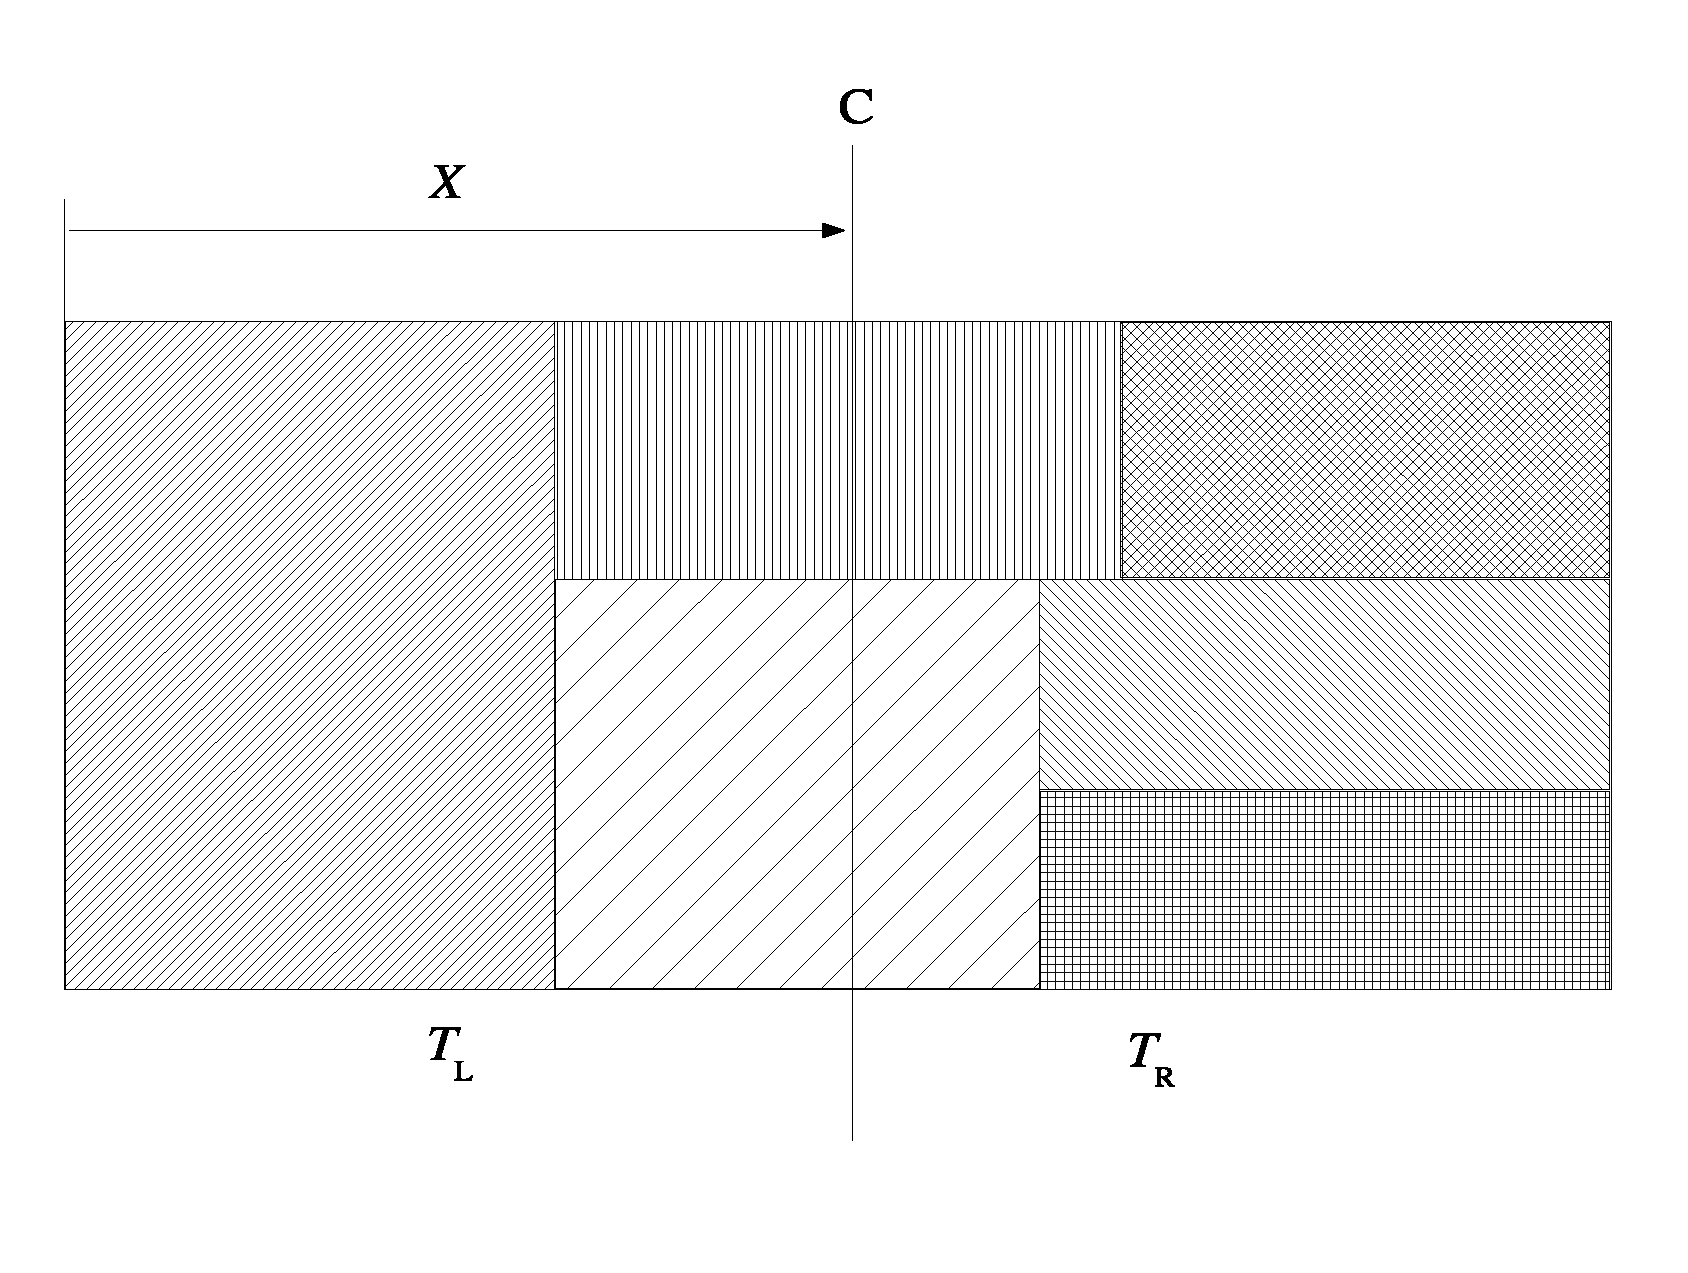
\includegraphics[clip]{ET.eps}}
\caption{A schematic diagram to illustrate the equal-time (ET) partitioning
scheme.  For simplicity a two-dimensional analog is used. The
rectangles represent the bounding ``boxes'' of the leaf nodes in a
CubeTree.  Different shades are used for different rectangles to indicate
that the leaf-node times are different in general. The distance of the
cutting line C from the left edge, $x$, is determined by the condition
that the sum of the leaf-node times on both sides of the partition line is
equal (i.e., $T_L = T_R$).  Notice that we have chosen the direction
for partitioning as the direction which gives the largest dimension.}
\label{fig:shiftline}
\end{figure}
% END FIGURE

Next we discuss the equal-time (ET) partitioning scheme, which is used
to repartition the root BBox based on the workload
information collected during the CubeTree construction in a particular
SCF cycle so that so that a better load balance will be achieved in
the next SCF calculation. In this way, the load information in the
$n$th SCF cycle will be used to load balance the computation of the
$(n+1)$th SCF cycle, for $n \ge 1$.  Through several experimentations,
we find the useful load information is the leaf-node time, which
measures the time to create a leaf node in a local CubeTree. The leaf-node
time includes the time to lay a grid in the BBox for the leaf node according to the 
cubature rules and evaluations of the density
and the density gradient on the leaf-node's grid. The
leaf-node time is collected during runtime and is stored along with
other attributes in a variable of type
CubeNode~\cite{Challacombe_00v113}.  It is important to notice that
the BBoxes of all leaf nodes on all processors will fill the root
BBox. The spatial distribution of all leaf nodes (which are spread
across all processors) will be very dense at places where a high resolution is
needed, and this will tend to have a higher workload. One might assume
that the workload is proportional to the number of leaf
nodes. However, we find we can do much better by assuming that the
workload is proportional to the sum of leaf-node times.
It should be remembered that the time
to create each leaf node will not be the same in general since the
environment (i.e. the portion of the RhoTree visited) that the BBox of a leaf
node experiences is generally different from all others.

Given that all processors hold the leaf-node times in their
respective local CubeTrees, the equal-time partitioning scheme creates
a new domain decomposition by recursively partitioning a box into two
subboxes such that each subbox carries approximately the same total
leaf-node times (hence the name ``equal-time'').  We have used a
robust bisection method~\cite{WPress92} to find the plane which
equally (to some threshold) divides the workload into half (see Figure
\ref{fig:shiftline}). Notice that the cutting direction may be varied
at each level of the recursion to avoid elongated subboxes which could
lead to poorly-balanced workloads. We have always chosen a direction
which cuts along the largest box dimension, since the cubature rules
will work best for near cube-like BBoxes for the leaf
nodes~\cite{Stroud71}.

It is important to point out that the working hypothesis of ET
partitioning scheme is that the sum of leaf-node times
for the root BBox is constant irrespective of the sectioning of the
root BBox.  In practice, this is not true since the total leaf-node
times will fluctuate if the cutting planes are shifted slightly. This
is because with each new partitioning, the adaptive grid will be
different. Since the time to create each leaf node depends on the
environment, the total leaf-node times will be different. However, it
is important to notice that the relative fluctuation of total
leaf-node times is small if the problem is coarse-grained. For very
fine-grained problems, relative fluctuations may be large and this
will create an imbalance problem, as will be seen in the results in
Section~\ref{sec:results}.

It is interesting to compare and contrast our ET repartitioning scheme
with other measurement based repartitioning schemes in the $N$-body
methods, such as the Orthogonal Recursive Bisection
(ORB)~\cite{warren:92_article} and the costzones
methods~\cite{Singh93}.  First we note the differences
between the ET partition and ORB.  In ET partition, we recursively split the 3D
space into many subspaces according to equal leaf-node times. However,
in the ORB for the Barnes-Hut
implementation~\cite{warren:92_article}, particles are grouped into groups
of particles.  This is achieved by partitioning the space containing
the particles with equal costs, where the costs correspond to the
number of interactions required to compute the force on the particles
in the space. It would be interesting to replace the cost counting in
ORB to the load timing information as in the ET partition, which may be more
appropriate since the time to compute each interaction might not be
the same in general.  In a costzones partitioning scheme~\cite{Singh93}, the {\it
tree} (rather than the 3D space) is partitioned 
with equal costs. The cost in the costzones method is defined in the
way as in the ORB.  So we concluded that ET partition
differs somewhat from ORB and costzones methods.  However, notice that
our ET partitioning scheme resembles the
ORB~\cite{warren:92_article} in the sense that both systematically section the work
space in varying directions.  In
Section~\ref{sec:implementation} we will show how both COM and ET
partitioning schemes may be incorporated into parallel HiCu with the
rest of the subroutines.

\section{Data parallel approach}
\label{sec:data-locality}
We have used a data parallel approach to implement parallel HiCu, in
anticipation of applications of our programs to very large systems
containing many atoms.  Data parallelism is an important issue because
naive data replication will exhaust the memory very quickly,
especially for very large systems. A data parallel approach is
possible because HiCu exhibits intrinsic data locality, which allows
us to use data parallel representation of the RhoTree, CubeTree, and
even $\Kxc$. The data parallel approach to these quantities will be
discussed in turn.  For HiCu, it is important to notice that each
subbox from a partitioning scheme has a well-defined boundary
(i.e. the six bounding planes), which means only the local information
about the electron density is needed.  By building a {\it locally
essential RhoTree}, which is {\it just}
sufficient to create the grid in a subbox, redundant replication of
data is avoided. Another advantage of a data parallel RhoTree is that
a traversal of a smaller locally essential RhoTree is more
efficient relative to a traversal of the entire RhoTree in the case of a
replicated density.

In a typical calculation, program {\tt MakeRho} will use the
row-distributed density matrix ${\bf P}^{P}$ ($P = 1, 2, \ldots, \Np$) 
to compute a distributed
intermediate Hermite-Gaussian (HG) ~\cite{Ahmadi95,Challacombe_00v113}
density.  Each process will independently calculate a set of density
distributions $\rho_q$ associated with only a number of rows
of ${\bf P}$. Each process will then save the
intermediate HG density distributions to its local disk, thus
spreading the data across many disks and avoiding hard disk
bottleneck. When parallel HiCu is invoked, each process will read the
intermediate HG density from its local disk.  It is important to
notice that the intermediate HG density, which is derived from
row-wise partitioning of the density matrix ${\bf P}$, is generally insufficient
to build a locally essential RhoTree for the subbox.  To
construct locally essential RhoTrees, all processes will go through
all local density distributions $\rho_q$ and use the information of
the dimensions of all other subboxes to determine if a local density
distribution $\rho_q$ needs to be sent to a remote process.
Once all local density distributions have been exchanged, each process
can build its own RhoTree which does not involve communications
between processes.  The construction of local CubeTrees follows,
which also involves no communication.

It is important to note that for a large system, $\Kxc$ is expected to
be sparse.  To facilitate efficient additions and updates of non-zero
matrix elements, we have designed a data structure called FastMat to store
the local $\Kxc$, denoted by ${\bf L}_{\mathrm{xc}}^{P}$, for $P = 1,
2, \ldots, \Np$.  In FastMat, all rows are connected by a linear
linked list, while each row is represented by a binary tree.  The
FastMat overcomes the inadequacy of the conventional blocked compressed
sparse row (BCSR) and distributed blocked compressed sparse row
(DBCSR) data structures, which do not allow random insertions and
updates of matrix elements.

We note that no communication between processes is needed when ${\bf
L}_{\mathrm{xc}}^{P}$ are computed.  The exchange-correlation matrix
$\Kxc$ is related to ${\bf L}_{\mathrm{xc}}^{P}$ by
\begin{equation}
\Kxc = \sum_{P=1}^{\Np}{\bf L}_{\mathrm{xc}}^{P}
\label{eq:kxcp}
\end{equation}
even though the summation in Eq.~(\ref{eq:kxcp}) has not been carried
out as a global sum in our program.  Instead, ${\bf
L}_{\mathrm{xc}}^{P} $ are redistributed to create row-wise
distributed ${\bf K}_{\mathrm{xc}}^{P}$, also stored in FastMat.  We
find that FastMat is also very useful for the redistribution of ${\bf
L}_{\mathrm{xc}}^{P}$ for ${\bf K}_{\mathrm{xc}}^{P}$,
since it involves insertions and updates of matrix
elements.  Our distribution approach should be contrasted with that
taken by Furlani {\it et al.}\/~\cite{Furlani_00v128} where
global summations to a single processor are performed. It should be
noted that parallel I/O is possible where ${{\bf
K}}_{\mathrm{xc}}^{P}$ may be written to separate disks for future
use.


\section{Implementation}
\label{sec:implementation}

\begin{figure}[t]
\resizebox*{3.5in}{!}{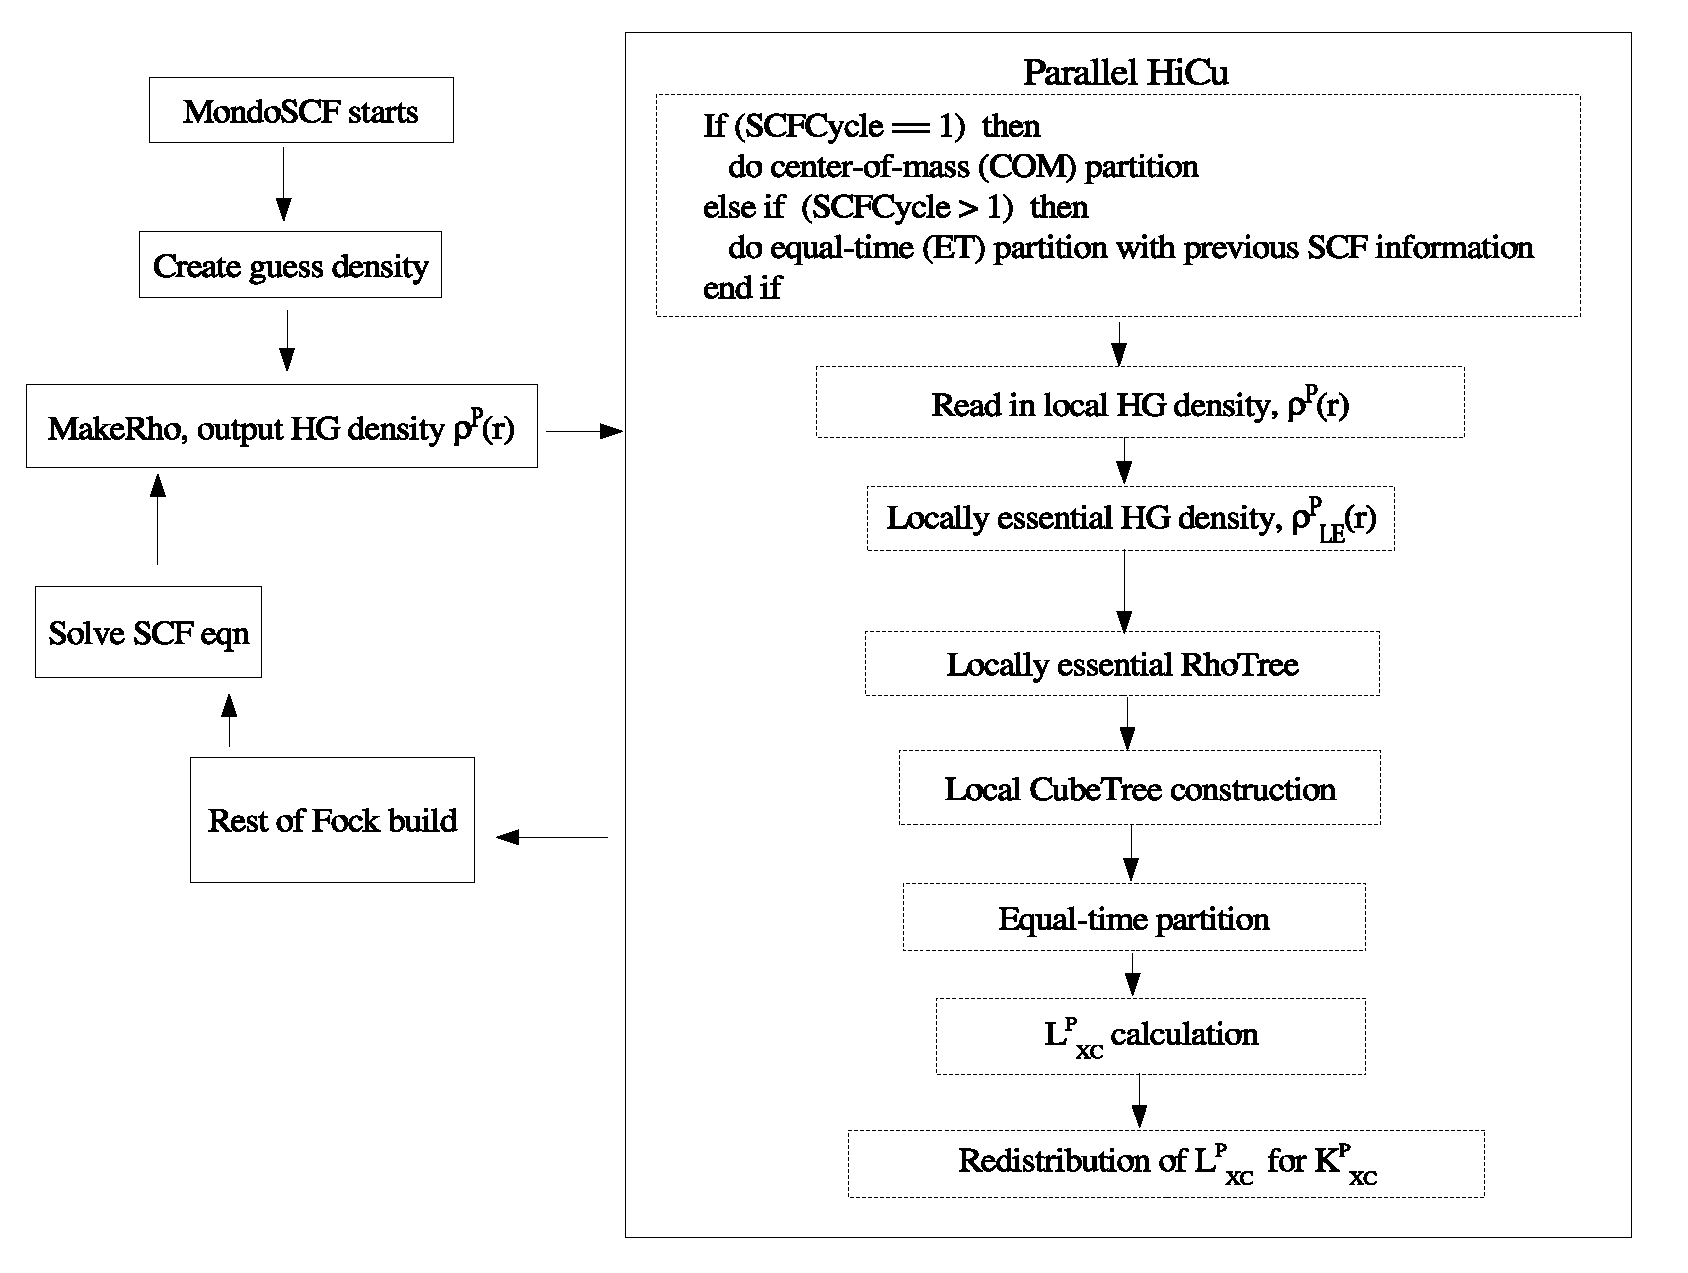
\includegraphics[clip]{PHiCuFlow.eps}}
\caption{The general flow of MondoSCF, with parallel HiCu subroutine
expanded.  Refer to Section~\ref{sec:implementation} for more
details.}
\label{fig:parahicu}
\end{figure}

We have implemented parallel HiCu in MondoSCF~\cite{Mondo}, a suite of
programs for linear scaling electronic structure theory and {\it ab
initio}\/ molecular dynamics.  Figure~\ref{fig:parahicu} shows the
general flow of MondoSCF, with an emphasis on parallel HiCu.  The
program {\tt MakeRho} is executed in parallel to calculate the
intermediate Hermite-Gaussian (HG) density distributions $\rho_q$ from
the row-wise distributed density matrix. If there are $\Np$ processes, 
then each process
will write a portion of the density distribution, $\rho^{P}({\bf
r})$, to its local disk, where $ P = 1, 2, \ldots, \Np$. When parallel
HiCu is invoked, one process will domain decompose the work space
(i.e. the root BBox) using either the center-of-mass partitioning
scheme at the first SCF cycle or the equal-time partitioning scheme at the
second or higher SCF cycles. The dimensions of subboxes after the
partitioning will be broadcast to all processors. Each process will
then load the intermediate HG density $\rho^{P}({\bf r})$,
from its local disk.  By going
through each density distribution $\rho_q$, a process will determine if a
distribution should be sent to other processes from the dimensions of
the subboxes. Some communications are needed to send the
necessary density distributions to other processes. Once a process
have all the essential density distributions, $\rho_{\mathrm{E}}^{P}({\bf r})$, 
a locally essential RhoTree is built.  Notice
that the locally essential RhoTrees are much smaller than the entire RhoTree in
the case of a replicated density.  Next local CubeTrees are built,
followed by an equal-time partition to facilitate repartitioning of
the root BBox in the next SCF cycle. The output of equal-time
partition is saved and will be used in the next SCF cycle.  Parallel
HiCu then proceeds with the calculation of local exchange-correlation
matrix, ${\bf L}_{\mathrm{xc}}^{P}$, which is related to $\Kxc$ by
Eq.~(\ref{eq:kxcp}).  To facilitate a full data parallel approach, we
redistribute ${\bf L}_{\mathrm{xc}}^{P}$ ($P = 1, 2, \ldots,\Np$) to
obtain row-wise distributed ${\bf K}_{\mathrm{xc}}^{P}$.

MondoSCF has been written in F95 with a message-passing paradigm using
the MPI library~\cite{mpi}.  The choice is made to ensure portability
of MondoSCF across different platforms and to free us from relying on
the underlying softwares and hardwares of the system.  More
importantly, the message-passing paradigm is used because as in many
parallel tree codes~\cite{Warren95b}, which involves dynamic and
irregular data structures, optimal performance can only be obtained by
having control over distribution and communication. We have used an
MPI function {\tt MPI\_WTIME} to calculate the leaf-node times.

%It is interesting to contrast our implementation approach with that used
%by Sosa {\it et al.}\/ They have used OpenMP to achieve parallelism,
%where user can fine-tune the codes via compiler directives or
%high-level command tools, which might need some experience.

\section{Results}
\label{sec:results}

We have performed scaling tests on taxol and a cluster of 110 water
molecules with $2^n$ processors, where $n$ typically ranges from 1 to
7.  These systems are chosen because they are highly inhomogeneous,
which pose a challenge for a good performance of the parallel HiCu.
All runs are performed on the SGI Origin 2000 with 250 MHz MIPS R10000
MIPS processors.  The result of the taxol scaling tests is shown in
Figure~\ref{fig:taxol}.
%The scaling results of taxol (which contains
%113 atoms) for 128-processor run is unavailable since MondoSCF
%requires each processor to hold at least one atom, which is not a
%severe restriction since large systems involving many atoms are the
%targets of MondoSCF.  
We start the calculation with a STO-3G basis set with a large $\tau$
threshold and then switch to 3-21G basis set and run for 3 SCF cycles.
The density matrix ${\bf P}$ is saved to the disk and scaling tests of
parallel HiCu are performed.  The procedure of switching the basis set
and iterating for a few SCF cycles is to ensure a typical electron density is
used.  The timings for parallel HiCu are taken at the fourth cycle
where the center-of-mass partition is used, and at the fifth cycle
where the equal-time partition is used.  Figure~\ref{fig:taxol}
shows that COM partitions perform rather poorly after 16 processors
where only a speedup of 22.4 is obtained with 64 processors.  However,
the equal-time partitions give good scaling results compared to the
ideal speedup, obtaining a speedup of 60.8 with 64 processors.  We
note that our result of a speedup of 7.03 with 8 processors compares
favorably with the speedup of about 6.0 of Sosa {\it et
al.}~\cite{Sosa_00v26}, which is for the single-point energy
calculation.

Similar scaling tests have been performed on a cluster of 110 water
molecules.  Figure~\ref{fig:waterscaling} shows that the
center-of-mass partition gives a better speedup than in the case of
taxol, presumably due to coarser-grained calculations.  The equal-time
repartitioning scheme is observed to be highly effective.  The speedup
is almost ideal up to 64 processors. We observe a superlinear speedup
at 32 processors, which corresponds to a medium-grained calculation.
We attribute the superlinear speedup as a result of a good load
balance as well as data parallelism, where the memory access time has been
greatly minimized since smaller trees are used.  The speedup with 128
processors degrades slightly, which is 112.64 (this corresponds to an
efficiency of 88\%).  But still this is an encouraging result because
the 128-processor run corresponds to very fine-grained parallelism,
where each processor handles about 1 heavy atom (oxygen). The reason
for a degraded efficiency for this very fine-grained calculation is
that an imbalance occurs due a relatively large fluctuation in the sum of
leaf-node times for each subbox, as explained in~
\ref{subsec:equal-time}.

Finally we note that SGI shared memory platform might not be ideal to
test our message-passing implementation of parallel HiCu. However, we
do not find a degradation of performance as shown by the results in
Figs.~\ref{fig:taxol} and \ref{fig:waterscaling}. This suggests that
the performance of parallel HiCu should be robust across different
platforms.

\section{Conclusions}
\label{sec:conclusions}
%approach.  Stratment. LinXC. and Jorda.  comment on
%\cite{Furlani_00v128,Sosa_98v19,Sosa_00v26}

We have proposed efficient parallelization of linear scaling
Hierarchical Cubature (HiCu) for numerical integration of
the exchange-correlation potential.  Both spatial and temporal localities
are exploited to domain decompose the work space, which is the volume
enclosing the electron density of the whole system.  The spatial locality has
been used to reduce communications between processors and to enable a
data parallel approach, which greatly reduce the memory usage and
facilitate efficient memory access since redundant information are not
stored.

To the best of our knowledge, we have proposed one of the first
measurement based strategies in quantum chemistry, called the
equal-time (ET) partitioning scheme, to perform domain decomposition
of the work space in all self-consistent-field cycles, except the first cycle.
This adaptive repartitioning scheme is proven to be highly effective
since we can exploit the temporal locality in a typical
self-consistent-field calculation. Even though the ET partitioning
scheme shares some ideas with the existing repartitioning schemes
for the tree implementations of the $N$-body methods, 
such as the Orthogonal Recursive Bisection (ORB)~\cite{warren:92_article} 
and costzones methods~\cite{Singh93}, the ET partition
differs from these two methods because (i) it partitions the 3D space (rather than
grouping the particles in ORB or partitioning the tree in costzones)
and (ii) exact load timing information is used (rather than counting the
number of interactions in $N$-body simulations in the ORB and costzones methods).

We have developed a new data structure FastMat to efficiently
facilitate insertions and updates of matrix elements, a feature which
is not found in the conventional blocked compressed sparse row (BCSR)
and distributed blocked compressed sparse row (DBCSR) data structures.

% Kxc and density matrix
It should be pointed out our parallelizations of $\Kxc$ differs
fundamentally from many existing parallelizations 
of $\Kxc$~\cite{Furlani_00v128,Yoshihiro_01v346}, which are
based on the original or modified Becke nuclear weight functions to
handle numerical integrations~\cite{Jorda95,Stratmann96,Scuseria99}. 
In most approaches~\cite{Furlani_00v128,Yoshihiro_01v346}, grid batches
are created and a simple master-slave dynamic loading balancing
scheme has been used. The master-slave scheme works 
well for a small number of slave programs
with coarse-grained parallelism.  However, unless a more sophisticated
dynamic loading balancing scheme is used, the simple master-slave scheme will not
give good scalings for fine-grained calculations with many processors,
since excessive communications between the master and the slave programs
will become the bottleneck of the calculations.

Our parallel HiCu code (in fact, all programs in MondoSCF) uses the intermediate 
Hermite-Gaussian densities~\cite{Ahmadi95,Challacombe_00v113}, which allows the
possibility of a data parallel approach. In this approach,
the row-distributed density matrix is used rather than the entire
density matrix~\cite{Furlani_00v128,Stratmann96,Sosa_00v26}, 
which can be prohibitively large to load onto any single processor
for very a large calculation.

Due to the use of advanced data structures to handle 
a dynamic irregular problem, we find
that the message-passing implementation of MPI gives us more control over 
distribution and communication. 
This will entail more programming efforts, however,
the efforts will be paid off with a highly efficient program, a conclusion
that has also been independently reached in Ref.~\cite{Warren95b}.

Due to a similar pattern of workload as in the $\Kxc$ calculation, the
exchange-correlation force calculation should lend itself to
straightforward parallelization.  Work is underway to parallelize HiCu
with periodic boundary conditions, which we expect
the equal-time partition should also work well.
Work is also underway to parallelize other parts of MondoSCF suite of
programs.  We expected the tree code experiences gained in parallel
HiCu would be valuable to parallelization of the Coulomb matrix
calculation with Quantum Chemistry Tree 
Code (QCTC)~\cite{Challacombe97,MChallacombe96,Challacombe96B}, which is another tree
code.

\begin{acknowledgments}
The Advanced Computing Laboratory of Los Alamos National Laboratory,
Los Alamos, New Mexico is acknowledged. Most of the calculations have
been performed on computing resources located at this facility.
\end{acknowledgments}

\bibliographystyle{apsrmp} \bibliography{mondo}

\begin{figure}[t]
\resizebox*{3.5in}{!}{\includegraphics[clip]{taxol_speedup.eps}}
\caption{Scaling of parallel HiCu on taxol (C$_{47}$H$_{51}$NO$_{14}$)
RHF/3-21G, with $\tau = 1.0 \times 10^{-6}$. The speedup for a
2-processor calculation is defined to be 2.}\label{fig:taxol}
\end{figure}

\begin{figure}[t]
\resizebox*{3.5in}{!}{\includegraphics[clip]{3-21G_good_div10.eps}}
\caption{Scaling of parallel HiCu on (H$_2$O)$_{110}$ RHF/3-21G, with
$\tau = 1.0 \times 10^{-6}$. The speedup for a 2-processor calculation
is defined to be 2.}
\label{fig:waterscaling}
\end{figure}

\end{document}
